\batchmode
\documentclass[twoside]{book}

% Packages required by doxygen
\usepackage{fixltx2e}
\usepackage{calc}
\usepackage{doxygen}
\usepackage[export]{adjustbox} % also loads graphicx
\usepackage{graphicx}
\usepackage[utf8]{inputenc}
\usepackage{makeidx}
\usepackage{multicol}
\usepackage{multirow}
\PassOptionsToPackage{warn}{textcomp}
\usepackage{textcomp}
\usepackage[nointegrals]{wasysym}
\usepackage[table]{xcolor}

% Font selection
\usepackage[T1]{fontenc}
\usepackage[scaled=.90]{helvet}
\usepackage{courier}
\usepackage{amssymb}
\usepackage{sectsty}
\renewcommand{\familydefault}{\sfdefault}
\allsectionsfont{%
  \fontseries{bc}\selectfont%
  \color{darkgray}%
}
\renewcommand{\DoxyLabelFont}{%
  \fontseries{bc}\selectfont%
  \color{darkgray}%
}
\newcommand{\+}{\discretionary{\mbox{\scriptsize$\hookleftarrow$}}{}{}}

% Page & text layout
\usepackage{geometry}
\geometry{%
  a4paper,%
  top=2.5cm,%
  bottom=2.5cm,%
  left=2.5cm,%
  right=2.5cm%
}
\tolerance=750
\hfuzz=15pt
\hbadness=750
\setlength{\emergencystretch}{15pt}
\setlength{\parindent}{0cm}
\setlength{\parskip}{3ex plus 2ex minus 2ex}
\makeatletter
\renewcommand{\paragraph}{%
  \@startsection{paragraph}{4}{0ex}{-1.0ex}{1.0ex}{%
    \normalfont\normalsize\bfseries\SS@parafont%
  }%
}
\renewcommand{\subparagraph}{%
  \@startsection{subparagraph}{5}{0ex}{-1.0ex}{1.0ex}{%
    \normalfont\normalsize\bfseries\SS@subparafont%
  }%
}
\makeatother

% Headers & footers
\usepackage{fancyhdr}
\pagestyle{fancyplain}
\fancyhead[LE]{\fancyplain{}{\bfseries\thepage}}
\fancyhead[CE]{\fancyplain{}{}}
\fancyhead[RE]{\fancyplain{}{\bfseries\leftmark}}
\fancyhead[LO]{\fancyplain{}{\bfseries\rightmark}}
\fancyhead[CO]{\fancyplain{}{}}
\fancyhead[RO]{\fancyplain{}{\bfseries\thepage}}
\fancyfoot[LE]{\fancyplain{}{}}
\fancyfoot[CE]{\fancyplain{}{}}
\fancyfoot[RE]{\fancyplain{}{\bfseries\scriptsize Generated by Doxygen }}
\fancyfoot[LO]{\fancyplain{}{\bfseries\scriptsize Generated by Doxygen }}
\fancyfoot[CO]{\fancyplain{}{}}
\fancyfoot[RO]{\fancyplain{}{}}
\renewcommand{\footrulewidth}{0.4pt}
\renewcommand{\chaptermark}[1]{%
  \markboth{#1}{}%
}
\renewcommand{\sectionmark}[1]{%
  \markright{\thesection\ #1}%
}

% Indices & bibliography
\usepackage{natbib}
\usepackage[titles]{tocloft}
\setcounter{tocdepth}{3}
\setcounter{secnumdepth}{5}
\makeindex

% Hyperlinks (required, but should be loaded last)
\usepackage{ifpdf}
\ifpdf
  \usepackage[pdftex,pagebackref=true]{hyperref}
\else
  \usepackage[ps2pdf,pagebackref=true]{hyperref}
\fi
\hypersetup{%
  colorlinks=true,%
  linkcolor=blue,%
  citecolor=blue,%
  unicode%
}

% Custom commands
\newcommand{\clearemptydoublepage}{%
  \newpage{\pagestyle{empty}\cleardoublepage}%
}

\usepackage{caption}
\captionsetup{labelsep=space,justification=centering,font={bf},singlelinecheck=off,skip=4pt,position=top}

%===== C O N T E N T S =====

\begin{document}

% Titlepage & ToC
\hypersetup{pageanchor=false,
             bookmarksnumbered=true,
             pdfencoding=unicode
            }
\pagenumbering{alph}
\pagenumbering{arabic}
\hypersetup{pageanchor=true}

%--- Begin generated contents ---
\chapter{Demo problem\+: Flow in a 2D channel with an elastic leaflet}
\label{index}\hypertarget{index}{}\hypertarget{index_q}{}\section{A few quick questions...}\label{index_q}
Since {\ttfamily oomph-\/lib} is developed as open-\/source software, any evidence that the code is being downloaded and used is very helpful for us as it helps to justify our continued work on this project.

We would therefore be extremely grateful if you could provide the information requested in the form below. Pressing the \char`\"{}submit\char`\"{} button will get you to the actual download page.

{\bfseries Note\+:} 
\begin{DoxyItemize}
\item All information will be treated as confidential. 
\item If you provide your email address and check the appropriate box we will add you to our mailing list to inform you of upgrades and bug fixes to the code. Rest assured that the mailing list is {\bfseries very low volume} -- we have better things to do than to bombard you with email. 
\item If you still feel reluctant to provide any of the information requested, feel free to enter some dummy input. The form will check that {\bfseries some} information has been entered but entering your name as \char`\"{}\+Joe Cool\char`\"{} is perfectly acceptable -- this is to discourage people from not providing the information simply because they are too lazy to type... 
\end{DoxyItemize}



 







 

 \hypertarget{index_pdf}{}\section{P\+D\+F file}\label{index_pdf}
A \href{../latex/refman.pdf}{\tt pdf version} of this document is available. \end{document}

\chapter{Namespace Index}
\section{Namespace List}
Here is a list of all namespaces with brief descriptions\+:\begin{DoxyCompactList}
\item\contentsline{section}{\hyperlink{namespaceGlobal__Physical__Variables}{Global\+\_\+\+Physical\+\_\+\+Variables} \\*Global variables that represent physical properties }{\pageref{namespaceGlobal__Physical__Variables}}{}
\item\contentsline{section}{\hyperlink{namespaceoomph}{oomph} }{\pageref{namespaceoomph}}{}
\item\contentsline{section}{\hyperlink{namespacePhysical__Variables}{Physical\+\_\+\+Variables} \\*Namespace for the solution of 2D linear shell equation }{\pageref{namespacePhysical__Variables}}{}
\end{DoxyCompactList}

\chapter{Hierarchical Index}
\section{Class Hierarchy}
This inheritance list is sorted roughly, but not completely, alphabetically\+:\begin{DoxyCompactList}
\item Problem\begin{DoxyCompactList}
\item \contentsline{section}{Unstructured\+Solid\+Problem$<$ E\+L\+E\+M\+E\+NT $>$}{\pageref{classUnstructuredSolidProblem}}{}
\end{DoxyCompactList}
\end{DoxyCompactList}

\chapter{Class Index}
\section{Class List}
Here are the classes, structs, unions and interfaces with brief descriptions\+:\begin{DoxyCompactList}
\item\contentsline{section}{\hyperlink{classPMLProblem}{P\+M\+L\+Problem$<$ E\+L\+E\+M\+E\+N\+T $>$} }{\pageref{classPMLProblem}}{}
\item\contentsline{section}{\hyperlink{classGlobalParameters_1_1TestPMLMapping}{Global\+Parameters\+::\+Test\+P\+M\+L\+Mapping} }{\pageref{classGlobalParameters_1_1TestPMLMapping}}{}
\end{DoxyCompactList}

\chapter{File Index}
\section{File List}
Here is a list of all files with brief descriptions\+:\begin{DoxyCompactList}
\item\contentsline{section}{\hyperlink{jeffery__orbit_8cc}{jeffery\+\_\+orbit.\+cc} }{\pageref{jeffery__orbit_8cc}}{}
\item\contentsline{section}{\hyperlink{jeffery__orbit_8txt__doxygenified_8h}{jeffery\+\_\+orbit.\+txt\+\_\+doxygenified.\+h} }{\pageref{jeffery__orbit_8txt__doxygenified_8h}}{}
\item\contentsline{section}{\hyperlink{my__taylor__hood__elements_8h}{my\+\_\+taylor\+\_\+hood\+\_\+elements.\+h} }{\pageref{my__taylor__hood__elements_8h}}{}
\end{DoxyCompactList}

\chapter{Namespace Documentation}
\hypertarget{namespaceGlobal__Physical__Variables}{}\section{Global\+\_\+\+Physical\+\_\+\+Variables Namespace Reference}
\label{namespaceGlobal__Physical__Variables}\index{Global\+\_\+\+Physical\+\_\+\+Variables@{Global\+\_\+\+Physical\+\_\+\+Variables}}


Namespace for physical parameters.  


\subsection*{Functions}
\begin{DoxyCompactItemize}
\item 
Vector$<$ double $>$ \hyperlink{namespaceGlobal__Physical__Variables_afae321364975eb56688ad13abc8ed6b7}{Gravity} (2)
\begin{DoxyCompactList}\small\item\em Gravity vector. \end{DoxyCompactList}\item 
void \hyperlink{namespaceGlobal__Physical__Variables_a87da705b8a46bed337cf5dbdd788b87b}{body\+\_\+force} (const double \&time, const Vector$<$ double $>$ \&x, Vector$<$ double $>$ \&result)
\begin{DoxyCompactList}\small\item\em Functional body force. \end{DoxyCompactList}\item 
void \hyperlink{namespaceGlobal__Physical__Variables_a9780d615ae07c4e00a436ab2973b54e6}{zero\+\_\+body\+\_\+force} (const double \&time, const Vector$<$ double $>$ \&x, Vector$<$ double $>$ \&result)
\begin{DoxyCompactList}\small\item\em Zero functional body force. \end{DoxyCompactList}\end{DoxyCompactItemize}
\subsection*{Variables}
\begin{DoxyCompactItemize}
\item 
double \hyperlink{namespaceGlobal__Physical__Variables_ab814e627d2eb5bc50318879d19ab16b9}{Re} =100
\begin{DoxyCompactList}\small\item\em Reynolds number. \end{DoxyCompactList}\item 
double \hyperlink{namespaceGlobal__Physical__Variables_ab1a845a672b4d74b304639a976dc65c6}{Re\+\_\+inv\+Fr} =100
\begin{DoxyCompactList}\small\item\em Reynolds/\+Froude number. \end{DoxyCompactList}\end{DoxyCompactItemize}


\subsection{Detailed Description}
Namespace for physical parameters. 

\subsection{Function Documentation}
\mbox{\Hypertarget{namespaceGlobal__Physical__Variables_a87da705b8a46bed337cf5dbdd788b87b}\label{namespaceGlobal__Physical__Variables_a87da705b8a46bed337cf5dbdd788b87b}} 
\index{Global\+\_\+\+Physical\+\_\+\+Variables@{Global\+\_\+\+Physical\+\_\+\+Variables}!body\+\_\+force@{body\+\_\+force}}
\index{body\+\_\+force@{body\+\_\+force}!Global\+\_\+\+Physical\+\_\+\+Variables@{Global\+\_\+\+Physical\+\_\+\+Variables}}
\subsubsection{\texorpdfstring{body\+\_\+force()}{body\_force()}}
{\footnotesize\ttfamily void Global\+\_\+\+Physical\+\_\+\+Variables\+::body\+\_\+force (\begin{DoxyParamCaption}\item[{const double \&}]{time,  }\item[{const Vector$<$ double $>$ \&}]{x,  }\item[{Vector$<$ double $>$ \&}]{result }\end{DoxyParamCaption})}



Functional body force. 



Definition at line 62 of file circular\+\_\+driven\+\_\+cavity.\+cc.



References Re\+\_\+inv\+Fr.



Referenced by main().

\mbox{\Hypertarget{namespaceGlobal__Physical__Variables_afae321364975eb56688ad13abc8ed6b7}\label{namespaceGlobal__Physical__Variables_afae321364975eb56688ad13abc8ed6b7}} 
\index{Global\+\_\+\+Physical\+\_\+\+Variables@{Global\+\_\+\+Physical\+\_\+\+Variables}!Gravity@{Gravity}}
\index{Gravity@{Gravity}!Global\+\_\+\+Physical\+\_\+\+Variables@{Global\+\_\+\+Physical\+\_\+\+Variables}}
\subsubsection{\texorpdfstring{Gravity()}{Gravity()}}
{\footnotesize\ttfamily Vector$<$double$>$ Global\+\_\+\+Physical\+\_\+\+Variables\+::\+Gravity (\begin{DoxyParamCaption}\item[{2}]{ }\end{DoxyParamCaption})}



Gravity vector. 



Referenced by main(), and Quarter\+Circle\+Driven\+Cavity\+Problem$<$ E\+L\+E\+M\+E\+N\+T $>$\+::\+Quarter\+Circle\+Driven\+Cavity\+Problem().

\mbox{\Hypertarget{namespaceGlobal__Physical__Variables_a9780d615ae07c4e00a436ab2973b54e6}\label{namespaceGlobal__Physical__Variables_a9780d615ae07c4e00a436ab2973b54e6}} 
\index{Global\+\_\+\+Physical\+\_\+\+Variables@{Global\+\_\+\+Physical\+\_\+\+Variables}!zero\+\_\+body\+\_\+force@{zero\+\_\+body\+\_\+force}}
\index{zero\+\_\+body\+\_\+force@{zero\+\_\+body\+\_\+force}!Global\+\_\+\+Physical\+\_\+\+Variables@{Global\+\_\+\+Physical\+\_\+\+Variables}}
\subsubsection{\texorpdfstring{zero\+\_\+body\+\_\+force()}{zero\_body\_force()}}
{\footnotesize\ttfamily void Global\+\_\+\+Physical\+\_\+\+Variables\+::zero\+\_\+body\+\_\+force (\begin{DoxyParamCaption}\item[{const double \&}]{time,  }\item[{const Vector$<$ double $>$ \&}]{x,  }\item[{Vector$<$ double $>$ \&}]{result }\end{DoxyParamCaption})}



Zero functional body force. 



Definition at line 70 of file circular\+\_\+driven\+\_\+cavity.\+cc.



Referenced by main().



\subsection{Variable Documentation}
\mbox{\Hypertarget{namespaceGlobal__Physical__Variables_ab814e627d2eb5bc50318879d19ab16b9}\label{namespaceGlobal__Physical__Variables_ab814e627d2eb5bc50318879d19ab16b9}} 
\index{Global\+\_\+\+Physical\+\_\+\+Variables@{Global\+\_\+\+Physical\+\_\+\+Variables}!Re@{Re}}
\index{Re@{Re}!Global\+\_\+\+Physical\+\_\+\+Variables@{Global\+\_\+\+Physical\+\_\+\+Variables}}
\subsubsection{\texorpdfstring{Re}{Re}}
{\footnotesize\ttfamily double Global\+\_\+\+Physical\+\_\+\+Variables\+::\+Re =100}



Reynolds number. 



Definition at line 53 of file circular\+\_\+driven\+\_\+cavity.\+cc.



Referenced by Quarter\+Circle\+Driven\+Cavity\+Problem$<$ E\+L\+E\+M\+E\+N\+T $>$\+::\+Quarter\+Circle\+Driven\+Cavity\+Problem().

\mbox{\Hypertarget{namespaceGlobal__Physical__Variables_ab1a845a672b4d74b304639a976dc65c6}\label{namespaceGlobal__Physical__Variables_ab1a845a672b4d74b304639a976dc65c6}} 
\index{Global\+\_\+\+Physical\+\_\+\+Variables@{Global\+\_\+\+Physical\+\_\+\+Variables}!Re\+\_\+inv\+Fr@{Re\+\_\+inv\+Fr}}
\index{Re\+\_\+inv\+Fr@{Re\+\_\+inv\+Fr}!Global\+\_\+\+Physical\+\_\+\+Variables@{Global\+\_\+\+Physical\+\_\+\+Variables}}
\subsubsection{\texorpdfstring{Re\+\_\+inv\+Fr}{Re\_invFr}}
{\footnotesize\ttfamily double Global\+\_\+\+Physical\+\_\+\+Variables\+::\+Re\+\_\+inv\+Fr =100}



Reynolds/\+Froude number. 



Definition at line 56 of file circular\+\_\+driven\+\_\+cavity.\+cc.



Referenced by body\+\_\+force(), and Quarter\+Circle\+Driven\+Cavity\+Problem$<$ E\+L\+E\+M\+E\+N\+T $>$\+::\+Quarter\+Circle\+Driven\+Cavity\+Problem().


\chapter{Class Documentation}
\hypertarget{classFSIChannelWithLeafletProblem}{}\section{F\+S\+I\+Channel\+With\+Leaflet\+Problem$<$ E\+L\+E\+M\+E\+NT $>$ Class Template Reference}
\label{classFSIChannelWithLeafletProblem}\index{F\+S\+I\+Channel\+With\+Leaflet\+Problem$<$ E\+L\+E\+M\+E\+N\+T $>$@{F\+S\+I\+Channel\+With\+Leaflet\+Problem$<$ E\+L\+E\+M\+E\+N\+T $>$}}
Inheritance diagram for F\+S\+I\+Channel\+With\+Leaflet\+Problem$<$ E\+L\+E\+M\+E\+NT $>$\+:\begin{figure}[H]
\begin{center}
\leavevmode
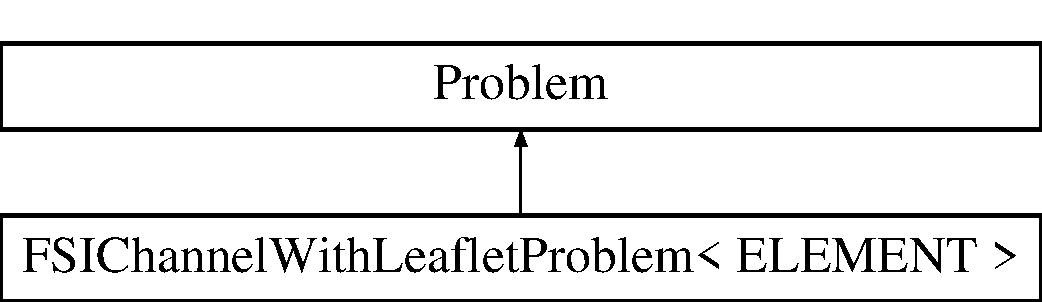
\includegraphics[height=2.000000cm]{classFSIChannelWithLeafletProblem}
\end{center}
\end{figure}
\subsection*{Public Member Functions}
\begin{DoxyCompactItemize}
\item 
\hyperlink{classFSIChannelWithLeafletProblem_a886599acf388d3ad5a2ec8c418c77280}{F\+S\+I\+Channel\+With\+Leaflet\+Problem} (const unsigned \&mesh\+\_\+multiplier)
\begin{DoxyCompactList}\small\item\em Constructor\+: Pass multiplier for uniform mesh refinement. \end{DoxyCompactList}\item 
\hyperlink{classFSIChannelWithLeafletProblem_a5df1d8f7229314a92ffb48ec61f56fe0}{$\sim$\+F\+S\+I\+Channel\+With\+Leaflet\+Problem} ()
\begin{DoxyCompactList}\small\item\em Destructor empty. \end{DoxyCompactList}\item 
void \hyperlink{classFSIChannelWithLeafletProblem_abff6e46a940263c9255a61f649bb4239}{actions\+\_\+after\+\_\+newton\+\_\+solve} ()
\begin{DoxyCompactList}\small\item\em Actions after solve (empty) \end{DoxyCompactList}\item 
void \hyperlink{classFSIChannelWithLeafletProblem_a8a32ef77f32b3283b4b509669deb0a11}{actions\+\_\+before\+\_\+newton\+\_\+solve} ()
\begin{DoxyCompactList}\small\item\em Actions before Newton solve\+: Reset the pseudo-\/elastic undeformed configuration. \end{DoxyCompactList}\item 
void \hyperlink{classFSIChannelWithLeafletProblem_aff02228eddae18ef3d57306ba1e61495}{actions\+\_\+before\+\_\+newton\+\_\+convergence\+\_\+check} ()
\begin{DoxyCompactList}\small\item\em Update no slip before Newton convergence check. \end{DoxyCompactList}\item 
void \hyperlink{classFSIChannelWithLeafletProblem_ac73220fa534cf2409bb0ebcf2fb5e1d5}{actions\+\_\+before\+\_\+implicit\+\_\+timestep} ()
\begin{DoxyCompactList}\small\item\em Actions before implicit timestep\+: Update the inflow velocity. \end{DoxyCompactList}\item 
void \hyperlink{classFSIChannelWithLeafletProblem_a8ca939c0edc4194e4e5cb7d1404f27de}{set\+\_\+iterative\+\_\+solver} ()
\begin{DoxyCompactList}\small\item\em Set iterative solver. \end{DoxyCompactList}\item 
void \hyperlink{classFSIChannelWithLeafletProblem_adca46cd909199b5721b6e17c15caae02}{doc\+\_\+solution} (Doc\+Info \&doc\+\_\+info)
\begin{DoxyCompactList}\small\item\em Doc the solution. \end{DoxyCompactList}\item 
void \hyperlink{classFSIChannelWithLeafletProblem_aa21f42ff019a517d94dbefdfc270c562}{create\+\_\+lagrange\+\_\+multiplier\+\_\+elements} ()
\begin{DoxyCompactList}\small\item\em Create elements that enforce prescribed boundary motion by Lagrange multipliers. \end{DoxyCompactList}\item 
void \hyperlink{classFSIChannelWithLeafletProblem_aeab2d2d99741e64d83792003db758c38}{delete\+\_\+lagrange\+\_\+multiplier\+\_\+elements} ()
\item 
void \hyperlink{classFSIChannelWithLeafletProblem_a27548bcf25ba14dca9f80ffcbc5792b0}{doc\+\_\+parameters} ()
\begin{DoxyCompactList}\small\item\em Doc parameters. \end{DoxyCompactList}\end{DoxyCompactItemize}
\subsection*{Private Member Functions}
\begin{DoxyCompactItemize}
\item 
Node $\ast$ \hyperlink{classFSIChannelWithLeafletProblem_a00605fef274ac93454d59b525ba4d923}{tip\+\_\+node\+\_\+pt} ()
\begin{DoxyCompactList}\small\item\em Helper fct; returns the node at the tip of the wall mesh. \end{DoxyCompactList}\end{DoxyCompactItemize}
\subsection*{Private Attributes}
\begin{DoxyCompactItemize}
\item 
Pseudo\+Elastic\+Channel\+With\+Leaflet\+Mesh$<$ E\+L\+E\+M\+E\+NT $>$ $\ast$ \hyperlink{classFSIChannelWithLeafletProblem_a336bdec3a8b90ac09feb89e5bb3539e8}{Bulk\+\_\+mesh\+\_\+pt}
\begin{DoxyCompactList}\small\item\em Pointer to the fluid mesh. \end{DoxyCompactList}\item 
One\+D\+Lagrangian\+Mesh$<$ F\+S\+I\+Hermite\+Beam\+Element $>$ $\ast$ \hyperlink{classFSIChannelWithLeafletProblem_a943437726f0a54fa8f7fc9ffb12bc4cd}{Wall\+\_\+mesh\+\_\+pt}
\begin{DoxyCompactList}\small\item\em Pointer to the \char`\"{}wall\char`\"{} mesh. \end{DoxyCompactList}\item 
B\+DF$<$ 2 $>$ $\ast$ \hyperlink{classFSIChannelWithLeafletProblem_ac58840d4c2fefae931eb55358099c28d}{Bulk\+\_\+time\+\_\+stepper\+\_\+pt}
\begin{DoxyCompactList}\small\item\em Bulk timestepper. \end{DoxyCompactList}\item 
Newmark$<$ 2 $>$ $\ast$ \hyperlink{classFSIChannelWithLeafletProblem_ace55d5753b8a32fcac448b8a45690afb}{Wall\+\_\+time\+\_\+stepper\+\_\+pt}
\begin{DoxyCompactList}\small\item\em Wall time stepper pt. \end{DoxyCompactList}\item 
Solid\+Mesh $\ast$ \hyperlink{classFSIChannelWithLeafletProblem_aab28704c88d14a2f0975ffcdfbe913e4}{Lagrange\+\_\+multiplier\+\_\+mesh\+\_\+pt}
\begin{DoxyCompactList}\small\item\em Pointers to mesh of Lagrange multiplier elements. \end{DoxyCompactList}\item 
Constitutive\+Law $\ast$ \hyperlink{classFSIChannelWithLeafletProblem_a745553864433ae6c0f1971776249193a}{Constitutive\+\_\+law\+\_\+pt}
\begin{DoxyCompactList}\small\item\em Constitutive law used to determine the mesh deformation. \end{DoxyCompactList}\item 
Mesh\+As\+Geom\+Object $\ast$ \hyperlink{classFSIChannelWithLeafletProblem_a2c6f28af7e78288f5b6d60f69036c8ee}{Wall\+\_\+geom\+\_\+object\+\_\+pt}
\begin{DoxyCompactList}\small\item\em Geometric object for the leaflet (to apply lagrange mult) \end{DoxyCompactList}\item 
\hyperlink{classUndeformedLeaflet}{Undeformed\+Leaflet} $\ast$ \hyperlink{classFSIChannelWithLeafletProblem_adb1d2ebc1379fac8b99cc61379d2b211}{Undeformed\+\_\+wall\+\_\+pt}
\begin{DoxyCompactList}\small\item\em Geom object for the leaflet. \end{DoxyCompactList}\end{DoxyCompactItemize}


\subsection{Detailed Description}
\subsubsection*{template$<$class E\+L\+E\+M\+E\+NT$>$\newline
class F\+S\+I\+Channel\+With\+Leaflet\+Problem$<$ E\+L\+E\+M\+E\+N\+T $>$}

F\+SI leaflet in channel. Mesh update with pseudo-\/elasticity and solved with pseudo-\/elastic fsi preconditioner. 

Definition at line 351 of file fsi\+\_\+channel\+\_\+with\+\_\+leaflet\+\_\+precond.\+cc.



\subsection{Constructor \& Destructor Documentation}
\mbox{\Hypertarget{classFSIChannelWithLeafletProblem_a886599acf388d3ad5a2ec8c418c77280}\label{classFSIChannelWithLeafletProblem_a886599acf388d3ad5a2ec8c418c77280}} 
\index{F\+S\+I\+Channel\+With\+Leaflet\+Problem@{F\+S\+I\+Channel\+With\+Leaflet\+Problem}!F\+S\+I\+Channel\+With\+Leaflet\+Problem@{F\+S\+I\+Channel\+With\+Leaflet\+Problem}}
\index{F\+S\+I\+Channel\+With\+Leaflet\+Problem@{F\+S\+I\+Channel\+With\+Leaflet\+Problem}!F\+S\+I\+Channel\+With\+Leaflet\+Problem@{F\+S\+I\+Channel\+With\+Leaflet\+Problem}}
\subsubsection{\texorpdfstring{F\+S\+I\+Channel\+With\+Leaflet\+Problem()}{FSIChannelWithLeafletProblem()}}
{\footnotesize\ttfamily template$<$class E\+L\+E\+M\+E\+NT $>$ \\
\hyperlink{classFSIChannelWithLeafletProblem}{F\+S\+I\+Channel\+With\+Leaflet\+Problem}$<$ E\+L\+E\+M\+E\+NT $>$\+::\hyperlink{classFSIChannelWithLeafletProblem}{F\+S\+I\+Channel\+With\+Leaflet\+Problem} (\begin{DoxyParamCaption}\item[{const unsigned \&}]{mesh\+\_\+multiplier }\end{DoxyParamCaption})}



Constructor\+: Pass multiplier for uniform mesh refinement. 

Constructor. 

Definition at line 494 of file fsi\+\_\+channel\+\_\+with\+\_\+leaflet\+\_\+precond.\+cc.



References Global\+\_\+\+Parameters\+::\+Fluid\+\_\+height, Global\+\_\+\+Parameters\+::\+Fluid\+\_\+length\+\_\+left, Global\+\_\+\+Parameters\+::\+Fluid\+\_\+length\+\_\+right, Global\+\_\+\+Parameters\+::H, Global\+\_\+\+Parameters\+::\+Lambda\+\_\+sq, Global\+\_\+\+Parameters\+::\+Lambda\+\_\+sq\+\_\+beam, Global\+\_\+\+Parameters\+::\+Leaflet\+\_\+height, Global\+\_\+\+Parameters\+::\+Leaflet\+\_\+x0, Global\+\_\+\+Parameters\+::\+Mesh\+\_\+nleft, Global\+\_\+\+Parameters\+::\+Mesh\+\_\+nright, Global\+\_\+\+Parameters\+::\+Mesh\+\_\+ny1, Global\+\_\+\+Parameters\+::\+Mesh\+\_\+ny2, Global\+\_\+\+Parameters\+::\+Nu, Global\+\_\+\+Parameters\+::Q, Global\+\_\+\+Parameters\+::\+Re, and Global\+\_\+\+Parameters\+::\+Re\+St.

\mbox{\Hypertarget{classFSIChannelWithLeafletProblem_a5df1d8f7229314a92ffb48ec61f56fe0}\label{classFSIChannelWithLeafletProblem_a5df1d8f7229314a92ffb48ec61f56fe0}} 
\index{F\+S\+I\+Channel\+With\+Leaflet\+Problem@{F\+S\+I\+Channel\+With\+Leaflet\+Problem}!````~F\+S\+I\+Channel\+With\+Leaflet\+Problem@{$\sim$\+F\+S\+I\+Channel\+With\+Leaflet\+Problem}}
\index{````~F\+S\+I\+Channel\+With\+Leaflet\+Problem@{$\sim$\+F\+S\+I\+Channel\+With\+Leaflet\+Problem}!F\+S\+I\+Channel\+With\+Leaflet\+Problem@{F\+S\+I\+Channel\+With\+Leaflet\+Problem}}
\subsubsection{\texorpdfstring{$\sim$\+F\+S\+I\+Channel\+With\+Leaflet\+Problem()}{~FSIChannelWithLeafletProblem()}}
{\footnotesize\ttfamily template$<$class E\+L\+E\+M\+E\+NT $>$ \\
\hyperlink{classFSIChannelWithLeafletProblem}{F\+S\+I\+Channel\+With\+Leaflet\+Problem}$<$ E\+L\+E\+M\+E\+NT $>$\+::$\sim$\hyperlink{classFSIChannelWithLeafletProblem}{F\+S\+I\+Channel\+With\+Leaflet\+Problem} (\begin{DoxyParamCaption}{ }\end{DoxyParamCaption})\hspace{0.3cm}{\ttfamily [inline]}}



Destructor empty. 



Definition at line 360 of file fsi\+\_\+channel\+\_\+with\+\_\+leaflet\+\_\+precond.\+cc.



\subsection{Member Function Documentation}
\mbox{\Hypertarget{classFSIChannelWithLeafletProblem_abff6e46a940263c9255a61f649bb4239}\label{classFSIChannelWithLeafletProblem_abff6e46a940263c9255a61f649bb4239}} 
\index{F\+S\+I\+Channel\+With\+Leaflet\+Problem@{F\+S\+I\+Channel\+With\+Leaflet\+Problem}!actions\+\_\+after\+\_\+newton\+\_\+solve@{actions\+\_\+after\+\_\+newton\+\_\+solve}}
\index{actions\+\_\+after\+\_\+newton\+\_\+solve@{actions\+\_\+after\+\_\+newton\+\_\+solve}!F\+S\+I\+Channel\+With\+Leaflet\+Problem@{F\+S\+I\+Channel\+With\+Leaflet\+Problem}}
\subsubsection{\texorpdfstring{actions\+\_\+after\+\_\+newton\+\_\+solve()}{actions\_after\_newton\_solve()}}
{\footnotesize\ttfamily template$<$class E\+L\+E\+M\+E\+NT $>$ \\
void \hyperlink{classFSIChannelWithLeafletProblem}{F\+S\+I\+Channel\+With\+Leaflet\+Problem}$<$ E\+L\+E\+M\+E\+NT $>$\+::actions\+\_\+after\+\_\+newton\+\_\+solve (\begin{DoxyParamCaption}{ }\end{DoxyParamCaption})\hspace{0.3cm}{\ttfamily [inline]}}



Actions after solve (empty) 



Definition at line 373 of file fsi\+\_\+channel\+\_\+with\+\_\+leaflet\+\_\+precond.\+cc.

\mbox{\Hypertarget{classFSIChannelWithLeafletProblem_ac73220fa534cf2409bb0ebcf2fb5e1d5}\label{classFSIChannelWithLeafletProblem_ac73220fa534cf2409bb0ebcf2fb5e1d5}} 
\index{F\+S\+I\+Channel\+With\+Leaflet\+Problem@{F\+S\+I\+Channel\+With\+Leaflet\+Problem}!actions\+\_\+before\+\_\+implicit\+\_\+timestep@{actions\+\_\+before\+\_\+implicit\+\_\+timestep}}
\index{actions\+\_\+before\+\_\+implicit\+\_\+timestep@{actions\+\_\+before\+\_\+implicit\+\_\+timestep}!F\+S\+I\+Channel\+With\+Leaflet\+Problem@{F\+S\+I\+Channel\+With\+Leaflet\+Problem}}
\subsubsection{\texorpdfstring{actions\+\_\+before\+\_\+implicit\+\_\+timestep()}{actions\_before\_implicit\_timestep()}}
{\footnotesize\ttfamily template$<$class E\+L\+E\+M\+E\+NT $>$ \\
void \hyperlink{classFSIChannelWithLeafletProblem}{F\+S\+I\+Channel\+With\+Leaflet\+Problem}$<$ E\+L\+E\+M\+E\+NT $>$\+::actions\+\_\+before\+\_\+implicit\+\_\+timestep (\begin{DoxyParamCaption}{ }\end{DoxyParamCaption})\hspace{0.3cm}{\ttfamily [inline]}}



Actions before implicit timestep\+: Update the inflow velocity. 



Definition at line 396 of file fsi\+\_\+channel\+\_\+with\+\_\+leaflet\+\_\+precond.\+cc.



References Global\+\_\+\+Parameters\+::\+Fluid\+\_\+height, and Global\+\_\+\+Parameters\+::flux().

\mbox{\Hypertarget{classFSIChannelWithLeafletProblem_aff02228eddae18ef3d57306ba1e61495}\label{classFSIChannelWithLeafletProblem_aff02228eddae18ef3d57306ba1e61495}} 
\index{F\+S\+I\+Channel\+With\+Leaflet\+Problem@{F\+S\+I\+Channel\+With\+Leaflet\+Problem}!actions\+\_\+before\+\_\+newton\+\_\+convergence\+\_\+check@{actions\+\_\+before\+\_\+newton\+\_\+convergence\+\_\+check}}
\index{actions\+\_\+before\+\_\+newton\+\_\+convergence\+\_\+check@{actions\+\_\+before\+\_\+newton\+\_\+convergence\+\_\+check}!F\+S\+I\+Channel\+With\+Leaflet\+Problem@{F\+S\+I\+Channel\+With\+Leaflet\+Problem}}
\subsubsection{\texorpdfstring{actions\+\_\+before\+\_\+newton\+\_\+convergence\+\_\+check()}{actions\_before\_newton\_convergence\_check()}}
{\footnotesize\ttfamily template$<$class E\+L\+E\+M\+E\+NT $>$ \\
void \hyperlink{classFSIChannelWithLeafletProblem}{F\+S\+I\+Channel\+With\+Leaflet\+Problem}$<$ E\+L\+E\+M\+E\+NT $>$\+::actions\+\_\+before\+\_\+newton\+\_\+convergence\+\_\+check (\begin{DoxyParamCaption}{ }\end{DoxyParamCaption})\hspace{0.3cm}{\ttfamily [inline]}}



Update no slip before Newton convergence check. 



Definition at line 384 of file fsi\+\_\+channel\+\_\+with\+\_\+leaflet\+\_\+precond.\+cc.

\mbox{\Hypertarget{classFSIChannelWithLeafletProblem_a8a32ef77f32b3283b4b509669deb0a11}\label{classFSIChannelWithLeafletProblem_a8a32ef77f32b3283b4b509669deb0a11}} 
\index{F\+S\+I\+Channel\+With\+Leaflet\+Problem@{F\+S\+I\+Channel\+With\+Leaflet\+Problem}!actions\+\_\+before\+\_\+newton\+\_\+solve@{actions\+\_\+before\+\_\+newton\+\_\+solve}}
\index{actions\+\_\+before\+\_\+newton\+\_\+solve@{actions\+\_\+before\+\_\+newton\+\_\+solve}!F\+S\+I\+Channel\+With\+Leaflet\+Problem@{F\+S\+I\+Channel\+With\+Leaflet\+Problem}}
\subsubsection{\texorpdfstring{actions\+\_\+before\+\_\+newton\+\_\+solve()}{actions\_before\_newton\_solve()}}
{\footnotesize\ttfamily template$<$class E\+L\+E\+M\+E\+NT $>$ \\
void \hyperlink{classFSIChannelWithLeafletProblem}{F\+S\+I\+Channel\+With\+Leaflet\+Problem}$<$ E\+L\+E\+M\+E\+NT $>$\+::actions\+\_\+before\+\_\+newton\+\_\+solve (\begin{DoxyParamCaption}{ }\end{DoxyParamCaption})\hspace{0.3cm}{\ttfamily [inline]}}



Actions before Newton solve\+: Reset the pseudo-\/elastic undeformed configuration. 



Definition at line 377 of file fsi\+\_\+channel\+\_\+with\+\_\+leaflet\+\_\+precond.\+cc.

\mbox{\Hypertarget{classFSIChannelWithLeafletProblem_aa21f42ff019a517d94dbefdfc270c562}\label{classFSIChannelWithLeafletProblem_aa21f42ff019a517d94dbefdfc270c562}} 
\index{F\+S\+I\+Channel\+With\+Leaflet\+Problem@{F\+S\+I\+Channel\+With\+Leaflet\+Problem}!create\+\_\+lagrange\+\_\+multiplier\+\_\+elements@{create\+\_\+lagrange\+\_\+multiplier\+\_\+elements}}
\index{create\+\_\+lagrange\+\_\+multiplier\+\_\+elements@{create\+\_\+lagrange\+\_\+multiplier\+\_\+elements}!F\+S\+I\+Channel\+With\+Leaflet\+Problem@{F\+S\+I\+Channel\+With\+Leaflet\+Problem}}
\subsubsection{\texorpdfstring{create\+\_\+lagrange\+\_\+multiplier\+\_\+elements()}{create\_lagrange\_multiplier\_elements()}}
{\footnotesize\ttfamily template$<$class E\+L\+E\+M\+E\+NT $>$ \\
void \hyperlink{classFSIChannelWithLeafletProblem}{F\+S\+I\+Channel\+With\+Leaflet\+Problem}$<$ E\+L\+E\+M\+E\+NT $>$\+::create\+\_\+lagrange\+\_\+multiplier\+\_\+elements (\begin{DoxyParamCaption}{ }\end{DoxyParamCaption})}



Create elements that enforce prescribed boundary motion by Lagrange multipliers. 

Create elements that impose the prescribed boundary displacement by Lagrange multipliers 

Definition at line 872 of file fsi\+\_\+channel\+\_\+with\+\_\+leaflet\+\_\+precond.\+cc.



References F\+S\+I\+Channel\+With\+Leaflet\+Problem$<$ E\+L\+E\+M\+E\+N\+T $>$\+::delete\+\_\+lagrange\+\_\+multiplier\+\_\+elements().



Referenced by F\+S\+I\+Channel\+With\+Leaflet\+Problem$<$ E\+L\+E\+M\+E\+N\+T $>$\+::set\+\_\+iterative\+\_\+solver().

\mbox{\Hypertarget{classFSIChannelWithLeafletProblem_aeab2d2d99741e64d83792003db758c38}\label{classFSIChannelWithLeafletProblem_aeab2d2d99741e64d83792003db758c38}} 
\index{F\+S\+I\+Channel\+With\+Leaflet\+Problem@{F\+S\+I\+Channel\+With\+Leaflet\+Problem}!delete\+\_\+lagrange\+\_\+multiplier\+\_\+elements@{delete\+\_\+lagrange\+\_\+multiplier\+\_\+elements}}
\index{delete\+\_\+lagrange\+\_\+multiplier\+\_\+elements@{delete\+\_\+lagrange\+\_\+multiplier\+\_\+elements}!F\+S\+I\+Channel\+With\+Leaflet\+Problem@{F\+S\+I\+Channel\+With\+Leaflet\+Problem}}
\subsubsection{\texorpdfstring{delete\+\_\+lagrange\+\_\+multiplier\+\_\+elements()}{delete\_lagrange\_multiplier\_elements()}}
{\footnotesize\ttfamily template$<$class E\+L\+E\+M\+E\+NT $>$ \\
void \hyperlink{classFSIChannelWithLeafletProblem}{F\+S\+I\+Channel\+With\+Leaflet\+Problem}$<$ E\+L\+E\+M\+E\+NT $>$\+::delete\+\_\+lagrange\+\_\+multiplier\+\_\+elements (\begin{DoxyParamCaption}{ }\end{DoxyParamCaption})}

Delete elements that enforce prescribed boundary motion by Lagrange multipliers

Delete elements that impose the prescribed boundary displacement and wipe the associated mesh 

Definition at line 947 of file fsi\+\_\+channel\+\_\+with\+\_\+leaflet\+\_\+precond.\+cc.



Referenced by F\+S\+I\+Channel\+With\+Leaflet\+Problem$<$ E\+L\+E\+M\+E\+N\+T $>$\+::create\+\_\+lagrange\+\_\+multiplier\+\_\+elements().

\mbox{\Hypertarget{classFSIChannelWithLeafletProblem_a27548bcf25ba14dca9f80ffcbc5792b0}\label{classFSIChannelWithLeafletProblem_a27548bcf25ba14dca9f80ffcbc5792b0}} 
\index{F\+S\+I\+Channel\+With\+Leaflet\+Problem@{F\+S\+I\+Channel\+With\+Leaflet\+Problem}!doc\+\_\+parameters@{doc\+\_\+parameters}}
\index{doc\+\_\+parameters@{doc\+\_\+parameters}!F\+S\+I\+Channel\+With\+Leaflet\+Problem@{F\+S\+I\+Channel\+With\+Leaflet\+Problem}}
\subsubsection{\texorpdfstring{doc\+\_\+parameters()}{doc\_parameters()}}
{\footnotesize\ttfamily template$<$class E\+L\+E\+M\+E\+NT $>$ \\
void \hyperlink{classFSIChannelWithLeafletProblem}{F\+S\+I\+Channel\+With\+Leaflet\+Problem}$<$ E\+L\+E\+M\+E\+NT $>$\+::doc\+\_\+parameters (\begin{DoxyParamCaption}{ }\end{DoxyParamCaption})\hspace{0.3cm}{\ttfamily [inline]}}



Doc parameters. 



Definition at line 432 of file fsi\+\_\+channel\+\_\+with\+\_\+leaflet\+\_\+precond.\+cc.



References Global\+\_\+\+Parameters\+::\+Lambda\+\_\+sq\+\_\+beam, Global\+\_\+\+Parameters\+::Q, Global\+\_\+\+Parameters\+::\+Re, and Global\+\_\+\+Parameters\+::T.

\mbox{\Hypertarget{classFSIChannelWithLeafletProblem_adca46cd909199b5721b6e17c15caae02}\label{classFSIChannelWithLeafletProblem_adca46cd909199b5721b6e17c15caae02}} 
\index{F\+S\+I\+Channel\+With\+Leaflet\+Problem@{F\+S\+I\+Channel\+With\+Leaflet\+Problem}!doc\+\_\+solution@{doc\+\_\+solution}}
\index{doc\+\_\+solution@{doc\+\_\+solution}!F\+S\+I\+Channel\+With\+Leaflet\+Problem@{F\+S\+I\+Channel\+With\+Leaflet\+Problem}}
\subsubsection{\texorpdfstring{doc\+\_\+solution()}{doc\_solution()}}
{\footnotesize\ttfamily template$<$class E\+L\+E\+M\+E\+NT $>$ \\
void \hyperlink{classFSIChannelWithLeafletProblem}{F\+S\+I\+Channel\+With\+Leaflet\+Problem}$<$ E\+L\+E\+M\+E\+NT $>$\+::doc\+\_\+solution (\begin{DoxyParamCaption}\item[{Doc\+Info \&}]{doc\+\_\+info }\end{DoxyParamCaption})}



Doc the solution. 



Definition at line 970 of file fsi\+\_\+channel\+\_\+with\+\_\+leaflet\+\_\+precond.\+cc.

\mbox{\Hypertarget{classFSIChannelWithLeafletProblem_a8ca939c0edc4194e4e5cb7d1404f27de}\label{classFSIChannelWithLeafletProblem_a8ca939c0edc4194e4e5cb7d1404f27de}} 
\index{F\+S\+I\+Channel\+With\+Leaflet\+Problem@{F\+S\+I\+Channel\+With\+Leaflet\+Problem}!set\+\_\+iterative\+\_\+solver@{set\+\_\+iterative\+\_\+solver}}
\index{set\+\_\+iterative\+\_\+solver@{set\+\_\+iterative\+\_\+solver}!F\+S\+I\+Channel\+With\+Leaflet\+Problem@{F\+S\+I\+Channel\+With\+Leaflet\+Problem}}
\subsubsection{\texorpdfstring{set\+\_\+iterative\+\_\+solver()}{set\_iterative\_solver()}}
{\footnotesize\ttfamily template$<$class E\+L\+E\+M\+E\+NT $>$ \\
void \hyperlink{classFSIChannelWithLeafletProblem}{F\+S\+I\+Channel\+With\+Leaflet\+Problem}$<$ E\+L\+E\+M\+E\+NT $>$\+::set\+\_\+iterative\+\_\+solver (\begin{DoxyParamCaption}{ }\end{DoxyParamCaption})}



Set iterative solver. 



Definition at line 737 of file fsi\+\_\+channel\+\_\+with\+\_\+leaflet\+\_\+precond.\+cc.



References F\+S\+I\+Channel\+With\+Leaflet\+Problem$<$ E\+L\+E\+M\+E\+N\+T $>$\+::create\+\_\+lagrange\+\_\+multiplier\+\_\+elements(), and L\+S\+C\+\_\+\+Preconditioner\+\_\+\+Helper\+::set\+\_\+hypre\+\_\+preconditioner().

\mbox{\Hypertarget{classFSIChannelWithLeafletProblem_a00605fef274ac93454d59b525ba4d923}\label{classFSIChannelWithLeafletProblem_a00605fef274ac93454d59b525ba4d923}} 
\index{F\+S\+I\+Channel\+With\+Leaflet\+Problem@{F\+S\+I\+Channel\+With\+Leaflet\+Problem}!tip\+\_\+node\+\_\+pt@{tip\+\_\+node\+\_\+pt}}
\index{tip\+\_\+node\+\_\+pt@{tip\+\_\+node\+\_\+pt}!F\+S\+I\+Channel\+With\+Leaflet\+Problem@{F\+S\+I\+Channel\+With\+Leaflet\+Problem}}
\subsubsection{\texorpdfstring{tip\+\_\+node\+\_\+pt()}{tip\_node\_pt()}}
{\footnotesize\ttfamily template$<$class E\+L\+E\+M\+E\+NT $>$ \\
Node$\ast$ \hyperlink{classFSIChannelWithLeafletProblem}{F\+S\+I\+Channel\+With\+Leaflet\+Problem}$<$ E\+L\+E\+M\+E\+NT $>$\+::tip\+\_\+node\+\_\+pt (\begin{DoxyParamCaption}{ }\end{DoxyParamCaption})\hspace{0.3cm}{\ttfamily [inline]}, {\ttfamily [private]}}



Helper fct; returns the node at the tip of the wall mesh. 



Definition at line 455 of file fsi\+\_\+channel\+\_\+with\+\_\+leaflet\+\_\+precond.\+cc.



\subsection{Member Data Documentation}
\mbox{\Hypertarget{classFSIChannelWithLeafletProblem_a336bdec3a8b90ac09feb89e5bb3539e8}\label{classFSIChannelWithLeafletProblem_a336bdec3a8b90ac09feb89e5bb3539e8}} 
\index{F\+S\+I\+Channel\+With\+Leaflet\+Problem@{F\+S\+I\+Channel\+With\+Leaflet\+Problem}!Bulk\+\_\+mesh\+\_\+pt@{Bulk\+\_\+mesh\+\_\+pt}}
\index{Bulk\+\_\+mesh\+\_\+pt@{Bulk\+\_\+mesh\+\_\+pt}!F\+S\+I\+Channel\+With\+Leaflet\+Problem@{F\+S\+I\+Channel\+With\+Leaflet\+Problem}}
\subsubsection{\texorpdfstring{Bulk\+\_\+mesh\+\_\+pt}{Bulk\_mesh\_pt}}
{\footnotesize\ttfamily template$<$class E\+L\+E\+M\+E\+NT $>$ \\
Pseudo\+Elastic\+Channel\+With\+Leaflet\+Mesh$<$E\+L\+E\+M\+E\+NT$>$$\ast$ \hyperlink{classFSIChannelWithLeafletProblem}{F\+S\+I\+Channel\+With\+Leaflet\+Problem}$<$ E\+L\+E\+M\+E\+NT $>$\+::Bulk\+\_\+mesh\+\_\+pt\hspace{0.3cm}{\ttfamily [private]}}



Pointer to the fluid mesh. 



Definition at line 463 of file fsi\+\_\+channel\+\_\+with\+\_\+leaflet\+\_\+precond.\+cc.

\mbox{\Hypertarget{classFSIChannelWithLeafletProblem_ac58840d4c2fefae931eb55358099c28d}\label{classFSIChannelWithLeafletProblem_ac58840d4c2fefae931eb55358099c28d}} 
\index{F\+S\+I\+Channel\+With\+Leaflet\+Problem@{F\+S\+I\+Channel\+With\+Leaflet\+Problem}!Bulk\+\_\+time\+\_\+stepper\+\_\+pt@{Bulk\+\_\+time\+\_\+stepper\+\_\+pt}}
\index{Bulk\+\_\+time\+\_\+stepper\+\_\+pt@{Bulk\+\_\+time\+\_\+stepper\+\_\+pt}!F\+S\+I\+Channel\+With\+Leaflet\+Problem@{F\+S\+I\+Channel\+With\+Leaflet\+Problem}}
\subsubsection{\texorpdfstring{Bulk\+\_\+time\+\_\+stepper\+\_\+pt}{Bulk\_time\_stepper\_pt}}
{\footnotesize\ttfamily template$<$class E\+L\+E\+M\+E\+NT $>$ \\
B\+DF$<$2$>$$\ast$ \hyperlink{classFSIChannelWithLeafletProblem}{F\+S\+I\+Channel\+With\+Leaflet\+Problem}$<$ E\+L\+E\+M\+E\+NT $>$\+::Bulk\+\_\+time\+\_\+stepper\+\_\+pt\hspace{0.3cm}{\ttfamily [private]}}



Bulk timestepper. 



Definition at line 469 of file fsi\+\_\+channel\+\_\+with\+\_\+leaflet\+\_\+precond.\+cc.

\mbox{\Hypertarget{classFSIChannelWithLeafletProblem_a745553864433ae6c0f1971776249193a}\label{classFSIChannelWithLeafletProblem_a745553864433ae6c0f1971776249193a}} 
\index{F\+S\+I\+Channel\+With\+Leaflet\+Problem@{F\+S\+I\+Channel\+With\+Leaflet\+Problem}!Constitutive\+\_\+law\+\_\+pt@{Constitutive\+\_\+law\+\_\+pt}}
\index{Constitutive\+\_\+law\+\_\+pt@{Constitutive\+\_\+law\+\_\+pt}!F\+S\+I\+Channel\+With\+Leaflet\+Problem@{F\+S\+I\+Channel\+With\+Leaflet\+Problem}}
\subsubsection{\texorpdfstring{Constitutive\+\_\+law\+\_\+pt}{Constitutive\_law\_pt}}
{\footnotesize\ttfamily template$<$class E\+L\+E\+M\+E\+NT $>$ \\
Constitutive\+Law$\ast$ \hyperlink{classFSIChannelWithLeafletProblem}{F\+S\+I\+Channel\+With\+Leaflet\+Problem}$<$ E\+L\+E\+M\+E\+NT $>$\+::Constitutive\+\_\+law\+\_\+pt\hspace{0.3cm}{\ttfamily [private]}}



Constitutive law used to determine the mesh deformation. 



Definition at line 478 of file fsi\+\_\+channel\+\_\+with\+\_\+leaflet\+\_\+precond.\+cc.

\mbox{\Hypertarget{classFSIChannelWithLeafletProblem_aab28704c88d14a2f0975ffcdfbe913e4}\label{classFSIChannelWithLeafletProblem_aab28704c88d14a2f0975ffcdfbe913e4}} 
\index{F\+S\+I\+Channel\+With\+Leaflet\+Problem@{F\+S\+I\+Channel\+With\+Leaflet\+Problem}!Lagrange\+\_\+multiplier\+\_\+mesh\+\_\+pt@{Lagrange\+\_\+multiplier\+\_\+mesh\+\_\+pt}}
\index{Lagrange\+\_\+multiplier\+\_\+mesh\+\_\+pt@{Lagrange\+\_\+multiplier\+\_\+mesh\+\_\+pt}!F\+S\+I\+Channel\+With\+Leaflet\+Problem@{F\+S\+I\+Channel\+With\+Leaflet\+Problem}}
\subsubsection{\texorpdfstring{Lagrange\+\_\+multiplier\+\_\+mesh\+\_\+pt}{Lagrange\_multiplier\_mesh\_pt}}
{\footnotesize\ttfamily template$<$class E\+L\+E\+M\+E\+NT $>$ \\
Solid\+Mesh$\ast$ \hyperlink{classFSIChannelWithLeafletProblem}{F\+S\+I\+Channel\+With\+Leaflet\+Problem}$<$ E\+L\+E\+M\+E\+NT $>$\+::Lagrange\+\_\+multiplier\+\_\+mesh\+\_\+pt\hspace{0.3cm}{\ttfamily [private]}}



Pointers to mesh of Lagrange multiplier elements. 



Definition at line 475 of file fsi\+\_\+channel\+\_\+with\+\_\+leaflet\+\_\+precond.\+cc.

\mbox{\Hypertarget{classFSIChannelWithLeafletProblem_adb1d2ebc1379fac8b99cc61379d2b211}\label{classFSIChannelWithLeafletProblem_adb1d2ebc1379fac8b99cc61379d2b211}} 
\index{F\+S\+I\+Channel\+With\+Leaflet\+Problem@{F\+S\+I\+Channel\+With\+Leaflet\+Problem}!Undeformed\+\_\+wall\+\_\+pt@{Undeformed\+\_\+wall\+\_\+pt}}
\index{Undeformed\+\_\+wall\+\_\+pt@{Undeformed\+\_\+wall\+\_\+pt}!F\+S\+I\+Channel\+With\+Leaflet\+Problem@{F\+S\+I\+Channel\+With\+Leaflet\+Problem}}
\subsubsection{\texorpdfstring{Undeformed\+\_\+wall\+\_\+pt}{Undeformed\_wall\_pt}}
{\footnotesize\ttfamily template$<$class E\+L\+E\+M\+E\+NT $>$ \\
\hyperlink{classUndeformedLeaflet}{Undeformed\+Leaflet}$\ast$ \hyperlink{classFSIChannelWithLeafletProblem}{F\+S\+I\+Channel\+With\+Leaflet\+Problem}$<$ E\+L\+E\+M\+E\+NT $>$\+::Undeformed\+\_\+wall\+\_\+pt\hspace{0.3cm}{\ttfamily [private]}}



Geom object for the leaflet. 



Definition at line 484 of file fsi\+\_\+channel\+\_\+with\+\_\+leaflet\+\_\+precond.\+cc.

\mbox{\Hypertarget{classFSIChannelWithLeafletProblem_a2c6f28af7e78288f5b6d60f69036c8ee}\label{classFSIChannelWithLeafletProblem_a2c6f28af7e78288f5b6d60f69036c8ee}} 
\index{F\+S\+I\+Channel\+With\+Leaflet\+Problem@{F\+S\+I\+Channel\+With\+Leaflet\+Problem}!Wall\+\_\+geom\+\_\+object\+\_\+pt@{Wall\+\_\+geom\+\_\+object\+\_\+pt}}
\index{Wall\+\_\+geom\+\_\+object\+\_\+pt@{Wall\+\_\+geom\+\_\+object\+\_\+pt}!F\+S\+I\+Channel\+With\+Leaflet\+Problem@{F\+S\+I\+Channel\+With\+Leaflet\+Problem}}
\subsubsection{\texorpdfstring{Wall\+\_\+geom\+\_\+object\+\_\+pt}{Wall\_geom\_object\_pt}}
{\footnotesize\ttfamily template$<$class E\+L\+E\+M\+E\+NT $>$ \\
Mesh\+As\+Geom\+Object$\ast$ \hyperlink{classFSIChannelWithLeafletProblem}{F\+S\+I\+Channel\+With\+Leaflet\+Problem}$<$ E\+L\+E\+M\+E\+NT $>$\+::Wall\+\_\+geom\+\_\+object\+\_\+pt\hspace{0.3cm}{\ttfamily [private]}}



Geometric object for the leaflet (to apply lagrange mult) 



Definition at line 481 of file fsi\+\_\+channel\+\_\+with\+\_\+leaflet\+\_\+precond.\+cc.

\mbox{\Hypertarget{classFSIChannelWithLeafletProblem_a943437726f0a54fa8f7fc9ffb12bc4cd}\label{classFSIChannelWithLeafletProblem_a943437726f0a54fa8f7fc9ffb12bc4cd}} 
\index{F\+S\+I\+Channel\+With\+Leaflet\+Problem@{F\+S\+I\+Channel\+With\+Leaflet\+Problem}!Wall\+\_\+mesh\+\_\+pt@{Wall\+\_\+mesh\+\_\+pt}}
\index{Wall\+\_\+mesh\+\_\+pt@{Wall\+\_\+mesh\+\_\+pt}!F\+S\+I\+Channel\+With\+Leaflet\+Problem@{F\+S\+I\+Channel\+With\+Leaflet\+Problem}}
\subsubsection{\texorpdfstring{Wall\+\_\+mesh\+\_\+pt}{Wall\_mesh\_pt}}
{\footnotesize\ttfamily template$<$class E\+L\+E\+M\+E\+NT $>$ \\
One\+D\+Lagrangian\+Mesh$<$F\+S\+I\+Hermite\+Beam\+Element$>$$\ast$ \hyperlink{classFSIChannelWithLeafletProblem}{F\+S\+I\+Channel\+With\+Leaflet\+Problem}$<$ E\+L\+E\+M\+E\+NT $>$\+::Wall\+\_\+mesh\+\_\+pt\hspace{0.3cm}{\ttfamily [private]}}



Pointer to the \char`\"{}wall\char`\"{} mesh. 



Definition at line 466 of file fsi\+\_\+channel\+\_\+with\+\_\+leaflet\+\_\+precond.\+cc.

\mbox{\Hypertarget{classFSIChannelWithLeafletProblem_ace55d5753b8a32fcac448b8a45690afb}\label{classFSIChannelWithLeafletProblem_ace55d5753b8a32fcac448b8a45690afb}} 
\index{F\+S\+I\+Channel\+With\+Leaflet\+Problem@{F\+S\+I\+Channel\+With\+Leaflet\+Problem}!Wall\+\_\+time\+\_\+stepper\+\_\+pt@{Wall\+\_\+time\+\_\+stepper\+\_\+pt}}
\index{Wall\+\_\+time\+\_\+stepper\+\_\+pt@{Wall\+\_\+time\+\_\+stepper\+\_\+pt}!F\+S\+I\+Channel\+With\+Leaflet\+Problem@{F\+S\+I\+Channel\+With\+Leaflet\+Problem}}
\subsubsection{\texorpdfstring{Wall\+\_\+time\+\_\+stepper\+\_\+pt}{Wall\_time\_stepper\_pt}}
{\footnotesize\ttfamily template$<$class E\+L\+E\+M\+E\+NT $>$ \\
Newmark$<$2$>$$\ast$ \hyperlink{classFSIChannelWithLeafletProblem}{F\+S\+I\+Channel\+With\+Leaflet\+Problem}$<$ E\+L\+E\+M\+E\+NT $>$\+::Wall\+\_\+time\+\_\+stepper\+\_\+pt\hspace{0.3cm}{\ttfamily [private]}}



Wall time stepper pt. 



Definition at line 472 of file fsi\+\_\+channel\+\_\+with\+\_\+leaflet\+\_\+precond.\+cc.



The documentation for this class was generated from the following file\+:\begin{DoxyCompactItemize}
\item 
\hyperlink{fsi__channel__with__leaflet__precond_8cc}{fsi\+\_\+channel\+\_\+with\+\_\+leaflet\+\_\+precond.\+cc}\end{DoxyCompactItemize}

\hypertarget{classUndeformedLeaflet}{}\section{Undeformed\+Leaflet Class Reference}
\label{classUndeformedLeaflet}\index{Undeformed\+Leaflet@{Undeformed\+Leaflet}}


Geom\+Object\+: Undeformed straight, vertical leaflet.  


Inheritance diagram for Undeformed\+Leaflet\+:\begin{figure}[H]
\begin{center}
\leavevmode
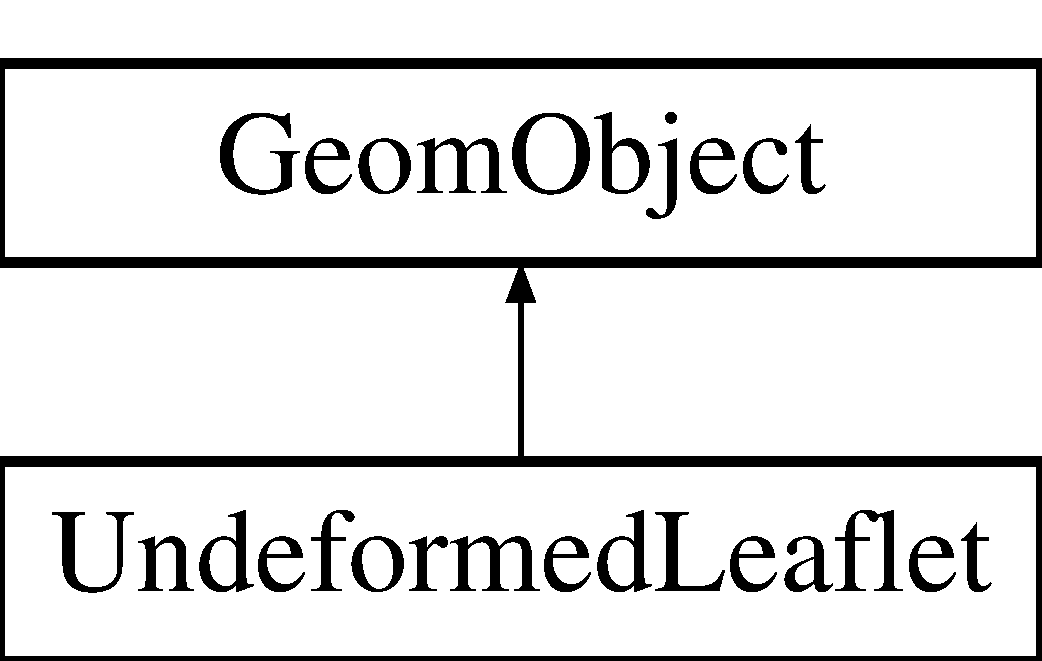
\includegraphics[height=2.000000cm]{classUndeformedLeaflet}
\end{center}
\end{figure}
\subsection*{Public Member Functions}
\begin{DoxyCompactItemize}
\item 
\hyperlink{classUndeformedLeaflet_ac4c0478b1f329360684af14b59043b12}{Undeformed\+Leaflet} (const double \&x0)
\begin{DoxyCompactList}\small\item\em Constructor\+: argument is the x-\/coordinate of the leaflet. \end{DoxyCompactList}\item 
void \hyperlink{classUndeformedLeaflet_a8e9b79702eb9a38e19886b84aeb47918}{position} (const Vector$<$ double $>$ \&zeta, Vector$<$ double $>$ \&r) const
\begin{DoxyCompactList}\small\item\em Position vector at Lagrangian coordinate zeta. \end{DoxyCompactList}\item 
void \hyperlink{classUndeformedLeaflet_a6949784da1030dd63ef741d170ef9798}{position} (const unsigned \&t, const Vector$<$ double $>$ \&zeta, Vector$<$ double $>$ \&r) const
\begin{DoxyCompactList}\small\item\em Parametrised position on object\+: r(zeta). Evaluated at previous timestep. t=0\+: current time; t$>$0\+: previous timestep. Calls steady version. \end{DoxyCompactList}\item 
void \hyperlink{classUndeformedLeaflet_a47d674756ce22e00a44ca0bd030a99da}{d2position} (const Vector$<$ double $>$ \&zeta, Vector$<$ double $>$ \&r, Dense\+Matrix$<$ double $>$ \&drdzeta, Rank\+Three\+Tensor$<$ double $>$ \&ddrdzeta) const
\begin{DoxyCompactList}\small\item\em Posn vector and its 1st \& 2nd derivatives w.\+r.\+t. to coordinates\+: $ \frac{dR_i}{d \zeta_\alpha}$ = drdzeta(alpha,i). $ \frac{d^2R_i}{d \zeta_\alpha d \zeta_\beta}$ = ddrdzeta(alpha,beta,i). Evaluated at current time. \end{DoxyCompactList}\item 
unsigned \hyperlink{classUndeformedLeaflet_a56153a1d117dd41657183655de094d3e}{ngeom\+\_\+data} () const
\begin{DoxyCompactList}\small\item\em Number of geometric Data in Geom\+Object\+: None. \end{DoxyCompactList}\end{DoxyCompactItemize}
\subsection*{Private Attributes}
\begin{DoxyCompactItemize}
\item 
double \hyperlink{classUndeformedLeaflet_aa89fc695af9e53aa38894c9d875afd36}{X0}
\begin{DoxyCompactList}\small\item\em x position of the undeformed leaflet\textquotesingle{}s origin. \end{DoxyCompactList}\end{DoxyCompactItemize}


\subsection{Detailed Description}
Geom\+Object\+: Undeformed straight, vertical leaflet. 

Definition at line 94 of file fsi\+\_\+channel\+\_\+with\+\_\+leaflet.\+cc.



\subsection{Constructor \& Destructor Documentation}
\mbox{\Hypertarget{classUndeformedLeaflet_ac4c0478b1f329360684af14b59043b12}\label{classUndeformedLeaflet_ac4c0478b1f329360684af14b59043b12}} 
\index{Undeformed\+Leaflet@{Undeformed\+Leaflet}!Undeformed\+Leaflet@{Undeformed\+Leaflet}}
\index{Undeformed\+Leaflet@{Undeformed\+Leaflet}!Undeformed\+Leaflet@{Undeformed\+Leaflet}}
\subsubsection{\texorpdfstring{Undeformed\+Leaflet()}{UndeformedLeaflet()}}
{\footnotesize\ttfamily Undeformed\+Leaflet\+::\+Undeformed\+Leaflet (\begin{DoxyParamCaption}\item[{const double \&}]{x0 }\end{DoxyParamCaption})\hspace{0.3cm}{\ttfamily [inline]}}



Constructor\+: argument is the x-\/coordinate of the leaflet. 



Definition at line 100 of file fsi\+\_\+channel\+\_\+with\+\_\+leaflet.\+cc.



\subsection{Member Function Documentation}
\mbox{\Hypertarget{classUndeformedLeaflet_a47d674756ce22e00a44ca0bd030a99da}\label{classUndeformedLeaflet_a47d674756ce22e00a44ca0bd030a99da}} 
\index{Undeformed\+Leaflet@{Undeformed\+Leaflet}!d2position@{d2position}}
\index{d2position@{d2position}!Undeformed\+Leaflet@{Undeformed\+Leaflet}}
\subsubsection{\texorpdfstring{d2position()}{d2position()}}
{\footnotesize\ttfamily void Undeformed\+Leaflet\+::d2position (\begin{DoxyParamCaption}\item[{const Vector$<$ double $>$ \&}]{zeta,  }\item[{Vector$<$ double $>$ \&}]{r,  }\item[{Dense\+Matrix$<$ double $>$ \&}]{drdzeta,  }\item[{Rank\+Three\+Tensor$<$ double $>$ \&}]{ddrdzeta }\end{DoxyParamCaption}) const\hspace{0.3cm}{\ttfamily [inline]}}



Posn vector and its 1st \& 2nd derivatives w.\+r.\+t. to coordinates\+: $ \frac{dR_i}{d \zeta_\alpha}$ = drdzeta(alpha,i). $ \frac{d^2R_i}{d \zeta_\alpha d \zeta_\beta}$ = ddrdzeta(alpha,beta,i). Evaluated at current time. 



Definition at line 130 of file fsi\+\_\+channel\+\_\+with\+\_\+leaflet.\+cc.

\mbox{\Hypertarget{classUndeformedLeaflet_a56153a1d117dd41657183655de094d3e}\label{classUndeformedLeaflet_a56153a1d117dd41657183655de094d3e}} 
\index{Undeformed\+Leaflet@{Undeformed\+Leaflet}!ngeom\+\_\+data@{ngeom\+\_\+data}}
\index{ngeom\+\_\+data@{ngeom\+\_\+data}!Undeformed\+Leaflet@{Undeformed\+Leaflet}}
\subsubsection{\texorpdfstring{ngeom\+\_\+data()}{ngeom\_data()}}
{\footnotesize\ttfamily unsigned Undeformed\+Leaflet\+::ngeom\+\_\+data (\begin{DoxyParamCaption}{ }\end{DoxyParamCaption}) const\hspace{0.3cm}{\ttfamily [inline]}}



Number of geometric Data in Geom\+Object\+: None. 



Definition at line 149 of file fsi\+\_\+channel\+\_\+with\+\_\+leaflet.\+cc.

\mbox{\Hypertarget{classUndeformedLeaflet_a8e9b79702eb9a38e19886b84aeb47918}\label{classUndeformedLeaflet_a8e9b79702eb9a38e19886b84aeb47918}} 
\index{Undeformed\+Leaflet@{Undeformed\+Leaflet}!position@{position}}
\index{position@{position}!Undeformed\+Leaflet@{Undeformed\+Leaflet}}
\subsubsection{\texorpdfstring{position()}{position()}\hspace{0.1cm}{\footnotesize\ttfamily [1/2]}}
{\footnotesize\ttfamily void Undeformed\+Leaflet\+::position (\begin{DoxyParamCaption}\item[{const Vector$<$ double $>$ \&}]{zeta,  }\item[{Vector$<$ double $>$ \&}]{r }\end{DoxyParamCaption}) const\hspace{0.3cm}{\ttfamily [inline]}}



Position vector at Lagrangian coordinate zeta. 



Definition at line 106 of file fsi\+\_\+channel\+\_\+with\+\_\+leaflet.\+cc.

\mbox{\Hypertarget{classUndeformedLeaflet_a6949784da1030dd63ef741d170ef9798}\label{classUndeformedLeaflet_a6949784da1030dd63ef741d170ef9798}} 
\index{Undeformed\+Leaflet@{Undeformed\+Leaflet}!position@{position}}
\index{position@{position}!Undeformed\+Leaflet@{Undeformed\+Leaflet}}
\subsubsection{\texorpdfstring{position()}{position()}\hspace{0.1cm}{\footnotesize\ttfamily [2/2]}}
{\footnotesize\ttfamily void Undeformed\+Leaflet\+::position (\begin{DoxyParamCaption}\item[{const unsigned \&}]{t,  }\item[{const Vector$<$ double $>$ \&}]{zeta,  }\item[{Vector$<$ double $>$ \&}]{r }\end{DoxyParamCaption}) const\hspace{0.3cm}{\ttfamily [inline]}}



Parametrised position on object\+: r(zeta). Evaluated at previous timestep. t=0\+: current time; t$>$0\+: previous timestep. Calls steady version. 



Definition at line 117 of file fsi\+\_\+channel\+\_\+with\+\_\+leaflet.\+cc.



\subsection{Member Data Documentation}
\mbox{\Hypertarget{classUndeformedLeaflet_aa89fc695af9e53aa38894c9d875afd36}\label{classUndeformedLeaflet_aa89fc695af9e53aa38894c9d875afd36}} 
\index{Undeformed\+Leaflet@{Undeformed\+Leaflet}!X0@{X0}}
\index{X0@{X0}!Undeformed\+Leaflet@{Undeformed\+Leaflet}}
\subsubsection{\texorpdfstring{X0}{X0}}
{\footnotesize\ttfamily double Undeformed\+Leaflet\+::\+X0\hspace{0.3cm}{\ttfamily [private]}}



x position of the undeformed leaflet\textquotesingle{}s origin. 



Definition at line 154 of file fsi\+\_\+channel\+\_\+with\+\_\+leaflet.\+cc.



The documentation for this class was generated from the following file\+:\begin{DoxyCompactItemize}
\item 
\hyperlink{fsi__channel__with__leaflet_8cc}{fsi\+\_\+channel\+\_\+with\+\_\+leaflet.\+cc}\end{DoxyCompactItemize}

\chapter{File Documentation}
\hypertarget{fsi__channel__with__leaflet_8cc}{}\section{fsi\+\_\+channel\+\_\+with\+\_\+leaflet.\+cc File Reference}
\label{fsi__channel__with__leaflet_8cc}\index{fsi\+\_\+channel\+\_\+with\+\_\+leaflet.\+cc@{fsi\+\_\+channel\+\_\+with\+\_\+leaflet.\+cc}}
\subsection*{Classes}
\begin{DoxyCompactItemize}
\item 
class \hyperlink{classUndeformedLeaflet}{Undeformed\+Leaflet}
\begin{DoxyCompactList}\small\item\em Geom\+Object\+: Undeformed straight, vertical leaflet. \end{DoxyCompactList}\item 
class \hyperlink{classFSIChannelWithLeafletProblem}{F\+S\+I\+Channel\+With\+Leaflet\+Problem$<$ E\+L\+E\+M\+E\+N\+T $>$}
\begin{DoxyCompactList}\small\item\em F\+SI leaflet in channel. \end{DoxyCompactList}\end{DoxyCompactItemize}
\subsection*{Namespaces}
\begin{DoxyCompactItemize}
\item 
 \hyperlink{namespaceGlobal__Physical__Variables}{Global\+\_\+\+Physical\+\_\+\+Variables}
\begin{DoxyCompactList}\small\item\em Global parameters. \end{DoxyCompactList}\end{DoxyCompactItemize}
\subsection*{Functions}
\begin{DoxyCompactItemize}
\item 
double \hyperlink{namespaceGlobal__Physical__Variables_ad651484fe06209606bccefe6fe23be0c}{Global\+\_\+\+Physical\+\_\+\+Variables\+::flux} (const double \&t)
\begin{DoxyCompactList}\small\item\em Flux\+: Pulsatile flow fluctuating between Min\+\_\+flux and Max\+\_\+flux with period Period. \end{DoxyCompactList}\item 
int \hyperlink{fsi__channel__with__leaflet_8cc_a0ddf1224851353fc92bfbff6f499fa97}{main} (int argc, char $\ast$argv\mbox{[}$\,$\mbox{]})
\end{DoxyCompactItemize}
\subsection*{Variables}
\begin{DoxyCompactItemize}
\item 
double \hyperlink{namespaceGlobal__Physical__Variables_ab814e627d2eb5bc50318879d19ab16b9}{Global\+\_\+\+Physical\+\_\+\+Variables\+::\+Re} =50.\+0
\begin{DoxyCompactList}\small\item\em Reynolds number. \end{DoxyCompactList}\item 
double \hyperlink{namespaceGlobal__Physical__Variables_a085ee4bf968ffdd01a41b8c41864f907}{Global\+\_\+\+Physical\+\_\+\+Variables\+::\+Re\+St} =50.\+0
\begin{DoxyCompactList}\small\item\em Womersley number\+: Product of Reynolds and Strouhal numbers. \end{DoxyCompactList}\item 
double \hyperlink{namespaceGlobal__Physical__Variables_af6e07423e22c0991084d9a2f43727805}{Global\+\_\+\+Physical\+\_\+\+Variables\+::H} =0.\+05
\begin{DoxyCompactList}\small\item\em Non-\/dimensional wall thickness. \end{DoxyCompactList}\item 
double \hyperlink{namespaceGlobal__Physical__Variables_a66cb7ecda9ba0cd72367dd697f154545}{Global\+\_\+\+Physical\+\_\+\+Variables\+::Q} =1.\+0e-\/6
\begin{DoxyCompactList}\small\item\em Fluid structure interaction parameter\+: Ratio of stresses used for non-\/dimensionalisation of fluid to solid stresses. \end{DoxyCompactList}\item 
double \hyperlink{namespaceGlobal__Physical__Variables_a2ffa220a56bff9b6b495ed47954d513f}{Global\+\_\+\+Physical\+\_\+\+Variables\+::\+Period} =2.\+0
\begin{DoxyCompactList}\small\item\em Period for fluctuations in flux. \end{DoxyCompactList}\item 
double \hyperlink{namespaceGlobal__Physical__Variables_aa46dc81a0757e8f9707646e03c32d4fc}{Global\+\_\+\+Physical\+\_\+\+Variables\+::\+Min\+\_\+flux} =1.\+0
\begin{DoxyCompactList}\small\item\em Min. flux. \end{DoxyCompactList}\item 
double \hyperlink{namespaceGlobal__Physical__Variables_aee645139728fd3d01573b161c74e7e8a}{Global\+\_\+\+Physical\+\_\+\+Variables\+::\+Max\+\_\+flux} =2.\+0
\begin{DoxyCompactList}\small\item\em Max. flux. \end{DoxyCompactList}\end{DoxyCompactItemize}


\subsection{Function Documentation}
\mbox{\Hypertarget{fsi__channel__with__leaflet_8cc_a0ddf1224851353fc92bfbff6f499fa97}\label{fsi__channel__with__leaflet_8cc_a0ddf1224851353fc92bfbff6f499fa97}} 
\index{fsi\+\_\+channel\+\_\+with\+\_\+leaflet.\+cc@{fsi\+\_\+channel\+\_\+with\+\_\+leaflet.\+cc}!main@{main}}
\index{main@{main}!fsi\+\_\+channel\+\_\+with\+\_\+leaflet.\+cc@{fsi\+\_\+channel\+\_\+with\+\_\+leaflet.\+cc}}
\subsubsection{\texorpdfstring{main()}{main()}}
{\footnotesize\ttfamily int main (\begin{DoxyParamCaption}\item[{int}]{argc,  }\item[{char $\ast$}]{argv\mbox{[}$\,$\mbox{]} }\end{DoxyParamCaption})}

Driver code -- pass a command line argument if you want to run the code in validation mode where it only performs a few steps 

Definition at line 760 of file fsi\+\_\+channel\+\_\+with\+\_\+leaflet.\+cc.



References Global\+\_\+\+Physical\+\_\+\+Variables\+::\+Re, and Global\+\_\+\+Physical\+\_\+\+Variables\+::\+Re\+St.


\hypertarget{fsi__channel__with__leaflet_8txt__doxygenified_8h}{}\section{fsi\+\_\+channel\+\_\+with\+\_\+leaflet.\+txt\+\_\+doxygenified.\+h File Reference}
\label{fsi__channel__with__leaflet_8txt__doxygenified_8h}\index{fsi\+\_\+channel\+\_\+with\+\_\+leaflet.\+txt\+\_\+doxygenified.\+h@{fsi\+\_\+channel\+\_\+with\+\_\+leaflet.\+txt\+\_\+doxygenified.\+h}}

%--- End generated contents ---

% Index
\backmatter
\newpage
\phantomsection
\clearemptydoublepage
\addcontentsline{toc}{chapter}{Index}
\printindex

\end{document}
